\documentclass[aspectratio=169]{Beamer} % Retire o aspectratio para adaptar a projetores antigos
\usepackage[utf8]{inputenc}		% Codificação do documento (conversão automática dos acentos)
\usepackage{color}				% Controle das cores
\usepackage{graphicx}			% Inclusão de gráficos
\usepackage[brazil]{babel}		% Idioma do documento
\usepackage{float} 				% Fixa tabelas e figuras no local exato
\usepackage{subfig}				% para inserir mais figuras
\usepackage{amsmath}			% para alguns formatos de equações
\usepackage{amssymb}			% para mais símbolos
\usepackage{animate}			% para gifs
\usepackage{pdflscape}			% Pdf landscape
\usepackage{pgfplots}
\usepackage{pgfplotstable}
\usepackage{tikz}
\usepackage{forest}
\usepackage{amsmath}
\usetikzlibrary{trees}
\usetikzlibrary{fit,shapes.arrows,positioning}

\tikzset{marrow/.style={midway,red,sloped,fill, minimum height=3cm, single arrow, single arrow
            head extend=.5cm, single arrow head indent=.25cm,xscale=0.3,yscale=0.15,
            allow upside down}}
%------	%------	%------	%------	%------	%------	%------	
\title[Especialização em Ciência de Dados e Big Data - ECD]{Análise de sentimentos em avaliações de clientes do \textit{e-commerce} nacional e comparação de métodos tradicionais de \textit{machine learning} com Redes Neurais \textit{Long Short Term Memory} (LSTM)}
%------	%------	%------	%------	%------	%------	%------	
\author[Carlos Magno de Brito]{{\Large Carlos Magno Santos Ribeiro de Brito}}
%------	%------	%------	%------	%------	%------	%------	
\institute[UFBA]{{\large Universidade Federal da Bahia}\\Departamento de Engenharia Elétrica e de Computação}
%------	%------	%------	%------	%------	%------	%------	
\date[UFBA 2023]

\logo{\includegraphics[width=0.8 cm]{logo_ufba.eps}}
\newcommand{\nologo}{\setbeamertemplate{logo}{}} % command to set the logo to nothing
%------	
\usetheme{CambridgeUS}
\usecolortheme{beaver}
%------ %------	%------	%------	%------	%------	%------
\usefonttheme[onlymath]{serif}	
%------ %------	%------	%------	%------	%------	%------
\begin{document}
% Definindo a capa
\frame{\titlepage}
% Definindo o sumário dividido na quantidade de slides necessária
\frame{\tableofcontents[part=1]}
% \frame{\tableofcontents[part=2]}
%------ %------	%------	%------	%------	%------	%------		
\part{1}
\section{Introdução}
\nologo
\frame{
    \frametitle{Introdução}
    \begin{itemize}
        \item O \textit{e-commerce} anualmente movimenta bilhões de dolares no mundo e está em franca expansão; \vskip1cm
        \item Os empreendimentos estão cada vez mais adotando tecnologias diversas em suas plataforma, inclusive lançando mão da ciência de dados para isso;\vskip1cm
        \item Para se manter competitiva e sólida neste mercado, uma empresa precisa de planejamento, inovação e, principalmente, entender sobre as necessidades dos clientes e como fidelizá-los;\vskip1cm
    \end{itemize}
}
\frame{
    \frametitle{Introdução}
    \begin{itemize}
        \item Uso de métodos do \textit{machine learning} e redes neurais surgem como opção para análise dos dados;\vskip1cm
        \item A depender do contexto, faz-se necessário utilizar métodos que sejam mais eficazes e consigam ter um \textit{tradeoff} entre tempo de processamento/acurácia satisfatório;\vskip1cm
        \item Foram utilizados quatro métodos tradicionais de aprendizado de máquina (Regressão logística, Naive Bayes, XGBoost e Florestas Aleatórias) e um modelo de rede neural artificial (LSTM) para fins comparativos.
    \end{itemize}
}
\subsection{Objetivos}
\frame{
    \frametitle{Objetivos}
    \begin{block}{Objetivo principal}
        Realizar análise com base de dados real sobre melhores modelos para se utilizar em estudo de satisfação dos consumidores em um comércio eletrônico
    \end{block}
    \begin{alertblock}{Objetivo secundário}
        \begin{itemize}
            \item Ponderar com a relação de eficiência \textit{versus} custo;
            \item Aplicar conceitos diversos da ciência/engenharia de dados, como por exemplo a mineração de texto, pré processamento e pós processamento de dados;
            \item Apresentar uma visão geral sobre o comércio eletrônico (e-commerce), sua evolução e importância no mercado brasileiro.
        \end{itemize}
    \end{alertblock}
}

\subsection{Justificativa}
\frame{
    \frametitle{Justificativa}
    Dentre as principais justificativas para o estudo dos \textit{e-commerces}, tem-se:\vskip0.5cm
    \begin{itemize}
        \item A análise de dados com essas técnicas pode ser feita de forma automatizada, reduzindo custos e tempo de processamento em comparação com análises manuais.;\vskip1cm
        \item Com essas técnicas é possível prever o comportamento dos consumidores, ajudando as empresas a tomarem decisões estratégicas;\vskip1cm
        \item A análise de dados com \textit{machine learning} e redes neurais pode ser aplicada em diferentes áreas do e-commerce, como marketing digital, o seu uso pode ajudar o negócio a otimizar o seu sistema logístico, reduzindo os custos de entrega e aumentando a satisfação dos clientes.
    \end{itemize}
}

\section{Materiais}
\frame{
    \frametitle{Tipo de pesquisa e descrição dos dados}
    \begin{itemize}
        \item A Olist é uma startup brasileira que atua no segmento de E-commerce por meio de marketplace.
        \item A empresa concentra vendedores que desejam anunciar em marketplaces como Mercado Livre, B2W, Via Varejo, Amazon, entre outros.
        \item A Olist concentra os produtos de todos os vendedores em uma loja única que fica visível ao consumidor final.
        \item Atualmente, a empresa reúne mais de 800 colaboradores e mais de 9 mil lojistas, além de 2 milhões de consumidores únicos.
        \item A base de dados escolhida para análise descreve a rotina de compra de um E-commerce e contém diversas informações sobre os produtos, como nome, preço, descrição, nota atribuída, comentários e local de compra.
        \item A análise se concentra especificamente nos comentários avaliativos (\textit{review comment message}) e nas notas dadas pelos clientes (\textit{review score}).
    \end{itemize}
}

\frame{
    \frametitle{Tipo de pesquisa e descrição dos dados}
    \begin{figure}[H]
        \centering
        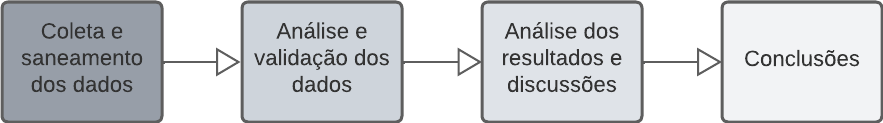
\includegraphics[width=\linewidth, scale=0.6]{../TCC/figs/process_diagram.png}
        \caption{Fluxograma do trabalho}
        \label{fig:process}
    \end{figure}
}
\frame{
    \frametitle{Exemplo da tabela usada}
    \begin{table}[H]
        \small
        \begin{tabular}{ccccc}
            \hline
            { }     & { review\_id}   & { order\_id}   & { review\_comment\_title} & { review\_comment\_message} \\ \hline
            { type} & { hash}         & { hash}        & { string|null}            & { string|null}              \\
            { ex}   & { da79b0a377eb} & { df73dbeba33} & { bom, mas}               & { atende às expectativas}   \\ \hline
        \end{tabular} \ldots
        \newline
        \vspace*{0.5 cm}
        \newline
        \begin{tabular}{cccc}
            \hline
            { }     & { review\_score} & { review\_creation\_date} & { review\_answer\_timestamp} \\ \hline
            { type} & { number}        & { datestring}             & { datestring}                \\
            { ex}   & { 3}             & { 2018-01-18 00:00:00}    & { 2018-01-18 21:00:00}       \\ \hline
        \end{tabular}
        \caption{Esquema da tabela \textit{olist\_order\_review}}
        \label{tab:review}
    \end{table}
}
\frame{
    \frametitle{Dataset utilizado}
    \begin{figure}[H]
        \centering
        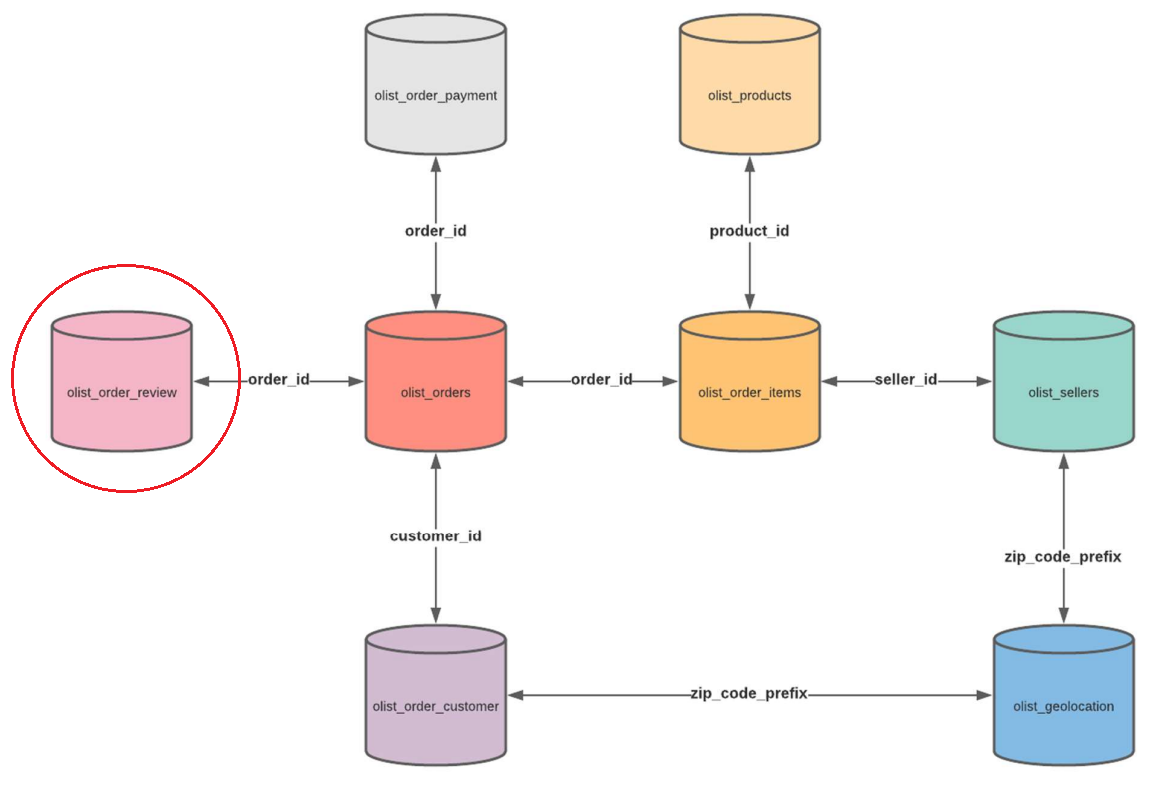
\includegraphics[scale=0.28]{../TCC/figs/database_schema.png}
        \caption{Esquemas do dataset publicado pelo Olist, adaptado pelo autor (2022)}
        \label{fig:dataset_schema}
    \end{figure}
}

\frame{
    \frametitle{Dataset transformado para uso}
    \begin{table}[H]
        \centering
        \begin{tabular}{cccc}
                    & index  & text               & label   \\\hline\hline
            type    & bigint & string             & boolean \\\hline
            exemplo & 1      & produto muito ruim & 0
        \end{tabular}
        \caption{Esquema de geração do \textit{data\_bin}}
        \label{tab:bin}
    \end{table}

    \begin{table}[H]
        \centering
        \begin{tabular}{cccc}
                    & index  & text              & label  \\\hline\hline
            type    & bigint & string            & number \\\hline
            exemplo & 2      & produto muito bom & 4
        \end{tabular}
        \caption{Esquema de geração do \textit{data\_gen}}
        \label{tab:gen}
    \end{table}

}
\frame{
    \begin{itemize}
        \item Os databases em formato CSV foram extraídos e exportados para leitura e armazenamento em diferentes variáveis.
        \item Itens duplicados, com valores nulos e valores discrepantes foram removidos.
        \item Separou-se dois \textit{datasets} contendo informações dos comentários dos clientes (\textit{review\_comment\_message}) e da sua nota de avaliação (\textit{review\_score}).
        \item Para o \textit{data\_bin} tem-se comentários associados categoricamente com valores binários (0 e 1) a partir das notas, com o valor atribuído de 0 para o intervalo $(0,2]$ e de 1 para o intervalo de $(2,5]$.
        \item No \textit{data\_cat} tem-se apenas os comentários e os reviews numéricos de 1 a 5.
        \item Ambas as bases são removidos os valores nulos.
    \end{itemize}
}

\subsubsection{Máquina para processamento}
\frame{
    \frametitle{Máquina para processamento}
    Todos os métodos foram executados em fila, sequencialmente entre eles, onde cada um deles foi executado em ordem, um de cada vez e de maneira procedural.

    A máquina utilizada para todos eles foi o laptop Dell G3 com processador Intel Core i7 de 10ª geração, 16GB de RAM, 512GB de SSD e placa de vídeo NVIDIA RTX 2060 com 6GB de memória dedicada, incluindo o sistema operacional Windows 11 com WSL 2 instalado e Ubuntu 20.04 como ambiente de execução para as ferramentas de teste de software usadas.
}



\section{Métodos}
\frame{
    \frametitle{Regressão Logística}
    \begin{itemize}
        \item A regressão logística é um modelo estatístico robusto e eficiente, que permite a previsão da probabilidade de um evento binário de forma precisa e confiável:
              \begin{enumerate}
                  \item Este tipo de evento é aquele que pode ocorrer ou não, ou que pode ser classificado em duas categorias distintas.
                  \item Por exemplo, em uma análise de crédito, o cliente pode ser aprovado ou não. Na medicina, o evento pode ser a cura ou não de uma doença.
              \end{enumerate}
        \item Ela apresenta um modelo linear generalizado que utiliza a função logística para modelar a relação entre as variáveis independentes e a variável dependente;
        \item A regressão logística utiliza a técnica de máxima verossimilhança para estimar os parâmetros do modelo a partir dos dados observados;
        \item A regressão logística tem sido amplamente utilizada em diversas áreas, como na análise de dados de sobrevivência, na análise de dados de saúde, na análise de dados financeiros, etc.
    \end{itemize}
}

\frame{
    \begin{figure}[H]
        \centering
        \begin{tikzpicture}
            \begin{axis}[    axis lines=left,    xlabel=$x$,    ylabel=$y$,    ymin=0, ymax=1,    ytick={0,1},    xmin=-5, xmax=5,    legend pos=north west]
                \addplot[domain=-5:5, samples=100, blue, thick] {1/(1+exp(-x))};
                \addlegendentry{$\frac{1}{1+e^{-x}}$};
                \draw[dashed] (axis cs:-5,0.5) -- (axis cs:5,0.5);
                \addplot[only marks, mark=*, red] coordinates {
                        (-4, 0.1)
                        (-1, 0.3)
                        (0, 0.6)
                        (1, 0.8)
                        (2, 0.9)
                        (4, 0.96)
                    };
                \addlegendentry{Dados}
            \end{axis}
        \end{tikzpicture}
        \caption{Modelo gráfico da regressão logística (curva sigmoide)}
        \label{plt:logistic}
    \end{figure}
}

\frame{
    \frametitle{Naive Bayes}
    \begin{itemize}
        \item A classificação Naive Bayes é um algoritmo de aprendizado de máquina supervisionado que utiliza o teorema de Bayes para classificar instâncias em classes discretas;
        \item A principal vantagem do algoritmo Naive Bayes é a sua simplicidade e eficiência computacional, o que o torna uma escolha popular para problemas de classificação em grande escala;
        \item O algoritmo Naive Bayes é baseado no teorema de Bayes, que fornece uma maneira de calcular a probabilidade condicional de uma hipótese, dado um conjunto de evidências;
        \item  A principal suposição por trás do algoritmo Naive Bayes é a independência condicional das características;
        \item O algoritmo Naive Bayes tem sido aplicado em muitas áreas, incluindo reconhecimento de fala, processamento de texto e detecção de spam de e-mail;
        \item Embora o algoritmo Naive Bayes seja uma técnica de classificação simples e eficiente, ele também tem algumas limitações.
    \end{itemize}

}

\begin{frame}
    \frametitle{Florestas Aleatórias}
    \begin{itemize}
        \item As florestas aleatórias são uma técnica de aprendizado de máquina que combina várias árvores de decisão para construir um modelo de classificação ou regressão.
        \item Cada árvore de decisão é construída a partir de um subconjunto aleatório dos dados de treinamento e um subconjunto aleatório dos recursos (também conhecidos como características ou atributos).
        \item A construção de uma árvore de decisão é feita por meio de uma série de etapas, onde a árvore começa com um único nó que representa todo o conjunto de dados de treinamento e é dividida em nós menores usando uma função de divisão que escolhe um recurso e um ponto de divisão que minimiza a impureza dos dados.
        \item Durante a fase de teste, a floresta aleatória retorna a classe mais comum ou a média das saídas das árvores individuais, dependendo se o problema é de classificação ou regressão, respectivamente.
        \item As florestas aleatórias apresentam várias vantagens em relação a outras técnicas de aprendizado de máquina, como bom desempenho em dados de alta dimensão, insensibilidade a outliers e dados ausentes e facilidade de paralelização.
        \item As florestas aleatórias são amplamente utilizadas em diversas áreas, como reconhecimento de padrões em imagens e sinais, detecção de fraudes em transações financeiras, análise de sentimentos em redes sociais, previsão de preços de ações e análise de dados genômicos.
    \end{itemize}
\end{frame}

\frame{
    \begin{figure}[H]
        \centering
        \scalebox{0.48}{
            \begin{forest}
                for tree={l sep=3em, s sep=3em, anchor=center, inner sep=0.7em, fill=blue!50,
                circle, font=\Large\sffamily,where level=1{no edge}{}}
                [Dados de treinamento, draw, rectangle, rounded corners, orange, text=white,alias=TD
                [,red!70,alias=a1[[,alias=a2][]][,red!70,edge label={node[above=1ex,marrow]{}}[[][]][,red!70,edge label={node[above=1ex,marrow]{}}[,red!70,edge label={node[below=1ex,marrow]{}}][,alias=a3]]]]
                [,red!70,alias=b1[,red!70,edge label={node[below=1ex,marrow]{}}[[,alias=b2][]][,red!70,edge label={node[above=1ex,marrow]{}}]][[][[][,alias=b3]]]]
                [~$\cdots$~,scale=4,no edge,fill=none,yshift=-1em]
                [,red!70,alias=c1[[,alias=c2][]][,red!70,edge label={node[above=1ex,marrow]{}}[,red!70,edge label={node[above=1ex,marrow]{}}[,alias=c3][,red!70,edge label={node[above=1ex,marrow]{}}]][,alias=c4]]]
                ]
                \node[draw,fit=(a1)(a2)(a3)](f1){};
                \node[draw,fit=(b1)(b2)(b3)](f2){};
                \node[draw,fit=(c1)(c2)(c3)(c4)](f3){};
                \path (f1.south west)--(f3.south east) node[midway,below=4em] (D) {Média};
                \node[below=2em of D] (pred){Predição};
                \foreach \X in {1,2,3}{\draw[-stealth] (TD) -- (f\X.north);
                        \draw[-stealth] (f\X.south) -- (D);}
                \draw[-stealth] (D) -- (pred);
            \end{forest}
        }
        \caption{Esquema de funcionamento de uma floresta aleatória}
        \label{plt:randomForest}
    \end{figure}
}

\frame{
    \frametitle{XGBoost}
    \begin{itemize}
        \item O XGBoost (\textit{Extreme Gradient Boosting}) é um método de aprendizado de máquina baseado em árvores de decisão, assim como as florestas aleatórias, mas com algumas diferenças importantes.
        \item Enquanto as florestas aleatórias usam um conjunto de árvores de decisão independentes para fazer uma previsão, o XGBoost usa um conjunto de árvores de decisão sequenciais que são criadas iterativamente. Cada nova árvore é ajustada aos resíduos do modelo anterior, tentando corrigir os erros cometidos pelo modelo atual.
        \item O algoritmo XGBoost foi desenvolvido por Tianqi Chen e Carlos Guestrin em 2016 e é baseado na biblioteca de código aberto de mesmo nome. O XGBoost se tornou um dos algoritmos de aprendizado de máquina mais populares em competições de ciência de dados e é amplamente utilizado na indústria.
        \item Para construir o modelo XGBoost, o algoritmo usa um processo iterativo de adição de árvores, onde cada nova árvore é ajustada aos resíduos do modelo anterior, tentando corrigir os erros cometidos pelo modelo atual.
    \end{itemize}

}

\frame{
    \frametitle{Redes Neurais LSTM}
    \begin{itemize}
        \item Uma rede neural artificial \textit{Long Short-Term Memory} (LSTM) é um tipo especializado de rede neural recorrente (RNN) projetada para lidar com o problema de dependência a longo prazo em sequências de dados.
        \item A principal característica da LSTM é a presença de unidades de memória, que são capazes de lembrar informações relevantes por um período prolongado de tempo.
        \item Essas unidades são compostas por três portões principais: o portão de entrada, o portão de esquecimento e o portão de saída.
    \end{itemize}
}

\frame{
    \frametitle{Redes Neurais LSTM}
    \begin{itemize}
        \item Durante o treinamento, a LSTM é capaz de aprender a modificar seus portões de entrada, esquecimento e saída, a fim de manter as informações relevantes na memória e descartar as informações irrelevantes.
        \item Os pesos das conexões entre as unidades de memória são atualizados usando o algoritmo de retropropagação através do tempo (BPTT).
        \item A arquitetura LSTM foi amplamente utilizada em diversas aplicações, incluindo processamento de linguagem natural, reconhecimento de fala e análise de séries temporais.
        \item Além disso, posteriormente foi proposta uma abordagem de aprendizado contínuo com LSTMs, chamada de "learning to forget", que permite que a rede esqueça informações irrelevantes à medida que recebe novos dados.
    \end{itemize}
}
\section{Resultados}
\frame{
    \frametitle{Distribuição}
    \begin{figure}[H]
        \centering
        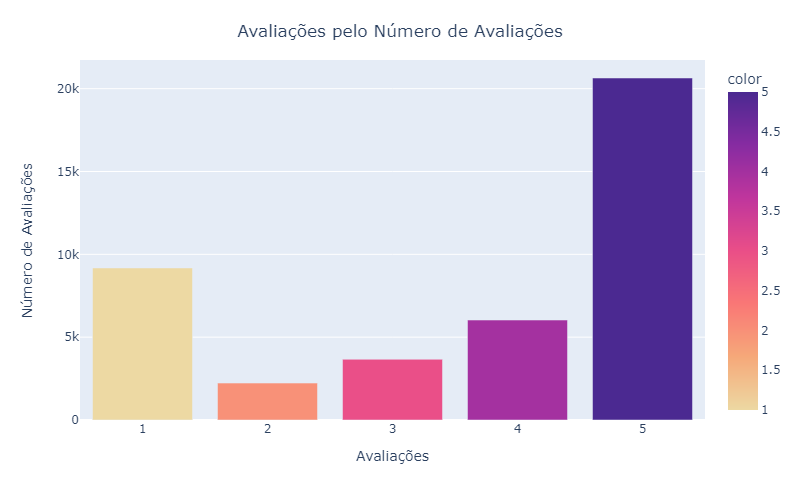
\includegraphics[trim={0cm 2cm 3cm 2cm},clip,scale=0.4]{../TCC/figs/eval.png}
        \caption{Distribuição das avaliações}
        \label{fig:evalDistribution}
    \end{figure}
}
\frame{
    \frametitle{Distribuição}
    \begin{figure}[H]
        \centering
        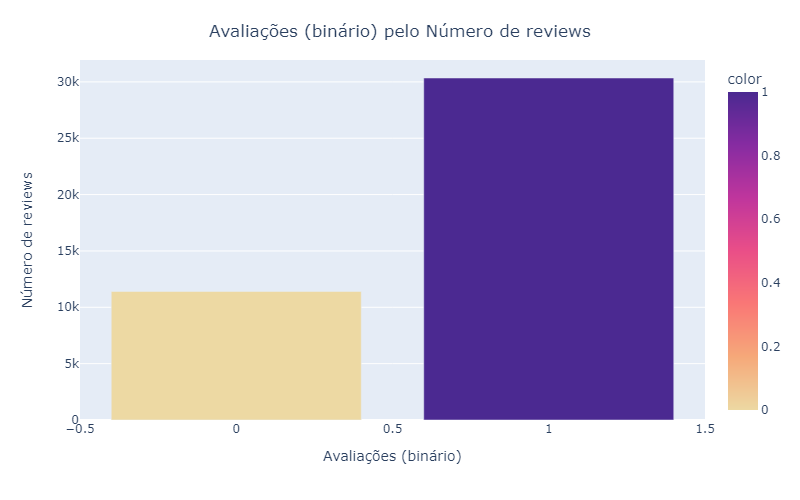
\includegraphics[trim={0cm 2cm 3cm 2cm},clip,scale=0.4]{../TCC/figs/bin_eval.png}
        \caption{Distribuição das avaliações binárias}
        \label{fig:binEvalDistribution}
    \end{figure}
}

\frame{
    \frametitle{Word Cloud}
    \begin{figure}[H]
        \centering
        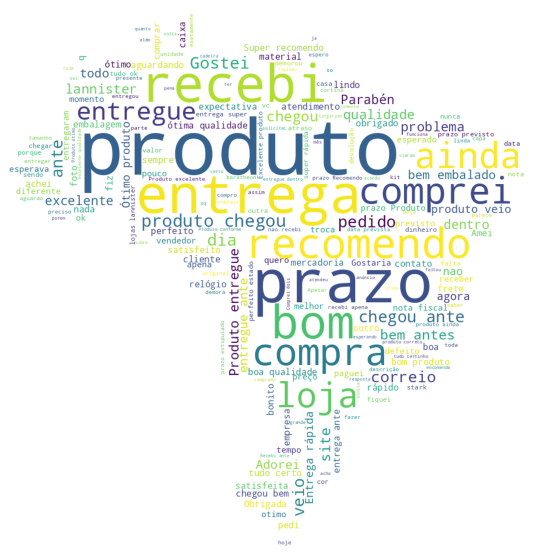
\includegraphics[scale=0.3]{../TCC/figs/word_cloud.png}
        \caption{Nuvem de palavras destacando os principais termos utilizados}
        \label{fig:wordCloud}
    \end{figure}
}

\frame{
    \frametitle{Acurácias}
    \begin{table}[H]
        \centering
        \begin{tabular}{l|cccc}
            \hline
            { modelo}      & { Reg. Logística} & { F. Aleatórias} & { XGBoost} & { Naive Bayes} \\ \hline\hline
            { treino (\%)} & { 73.9}           & { 99.6}          & { 93.5}    & { 74.0}        \\\hline
            { teste (\%)}  & { 73.3}           & { 78.2}          & { 82.1}    & { 74.0}
        \end{tabular}
    \end{table}
}

\frame{
    \frametitle{Acurácias}
    \begin{figure}[H]
        \centering
        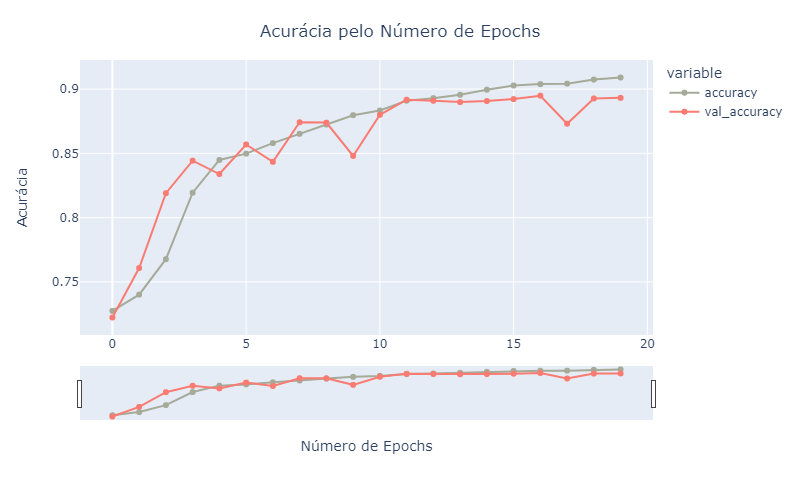
\includegraphics[scale=0.35]{../TCC/figs/lstm_acuracy.png}
        \caption{Relação acurácia por \textit{epochs}}
        \label{fig:lstmacuracy}
    \end{figure}
}

\frame{
    \frametitle{Acurácias}
    \begin{figure}[H]
        \centering
        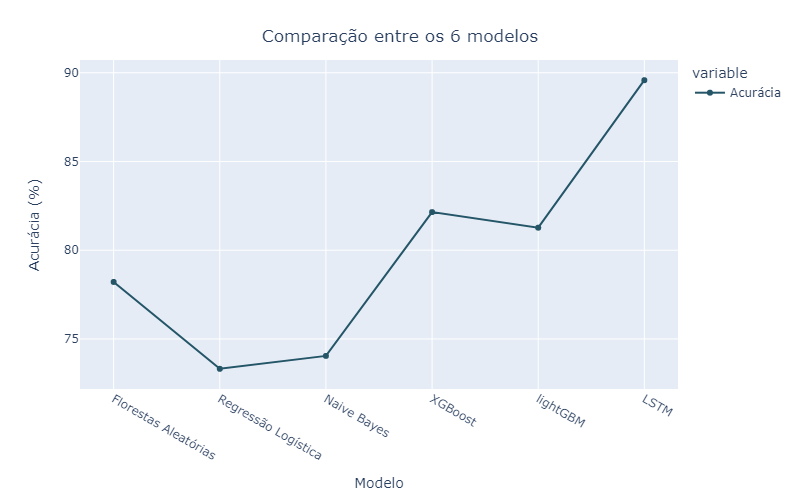
\includegraphics[scale=0.35]{../TCC/figs/comparative.png}
        \caption{Comparação de acurácia entre modelos}
        \label{fig:comparative}
    \end{figure}
}

\frame{
    \frametitle{\textit{Tradeoff}}
    \begin{table}[H]
        \centering
        \begin{tabular}{c|ccccl}
            \hline
            { modelo}        & { Reg. Logística} & { F. Aleatórias} & { XGBoost} & { Naive Bayes} & LSTM \\ \hline \hline
            { Tempo (s)}     & { 21.5}           & { 1.5}           & { 3.0}     & { 0.1}         & 1500 \\ \hline
            { Acurácia (\%)} & { 73.3}           & { 78.2}          & { 82.1}    & { 74.0}        & 90.0 \\
        \end{tabular}
        \caption{Tempo de execução/Acurácia dos modelos avaliados}
        \label{tab:time}
    \end{table}
}

\frame{
    \frametitle{Matriz de confusão}
    \begin{figure}[H]
        \centering
        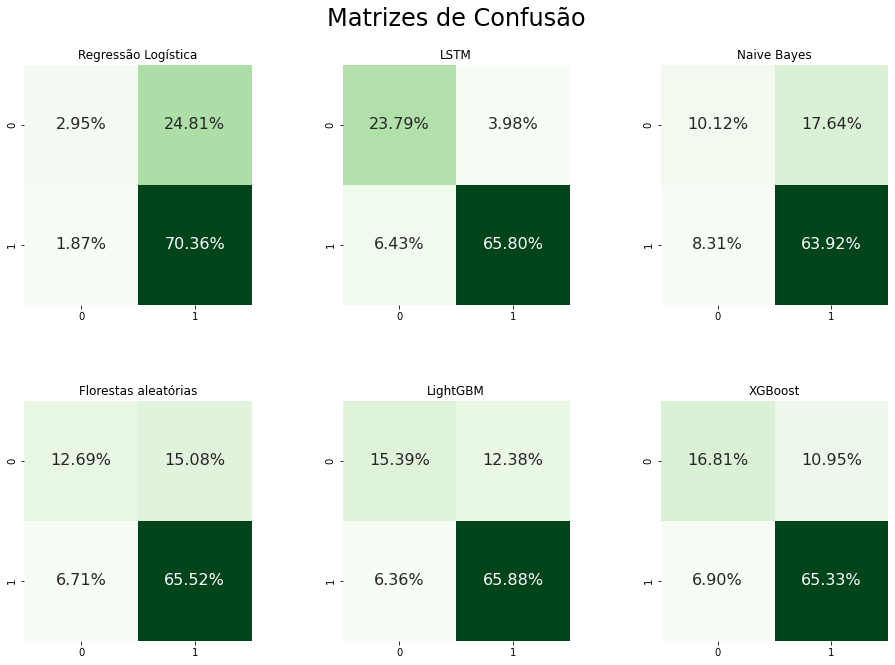
\includegraphics[scale=0.25]{../TCC/figs/confusion.png}
        \caption{Curvas ROC dos modelos utilizados}
        \label{fig:roccurve}
    \end{figure}
}

\frame{
    \frametitle{Curva HOC}
    \begin{figure}[H]
        \centering
        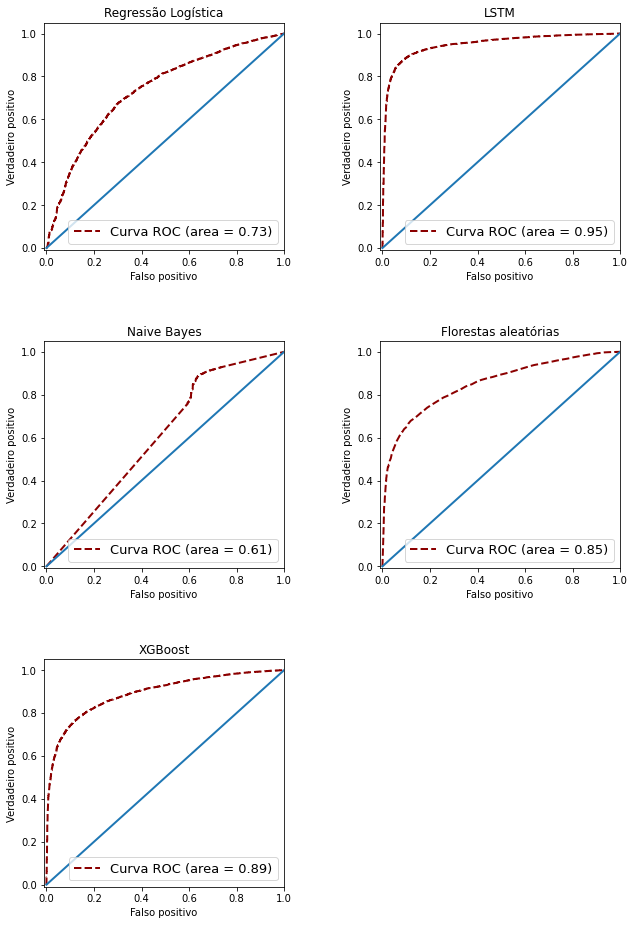
\includegraphics[scale=0.3]{../TCC/figs/roc.png}
        \caption{Matrizes de confusão dos modelos utilizados}
        \label{fig:mconfusion}
    \end{figure}
}




\section{Conclusões}
\frame{
    \frametitle{Conclusões}
    \begin{itemize}
        \item A Rede neural LSTM apresentou a melhor performance entre os algoritmos de machine learning avaliados, com acurácia de $90\%$ e maior capacidade de distinguir entre as classes, indicado pela área sob a curva ROC.

        \item XGBoost também apresentou resultados promissores, com acurácia de $82\%$ e área sob a curva ROC de 0,89, mas cometeu mais erros na classificação de algumas amostras do que a LSTM.

        \item Regressão logística e Naive Bayes tiveram as piores performances, com acurácias de $73\%$ e $61\%$, respectivamente, e áreas sob a curva ROC menores do que os outros modelos avaliados.
    \end{itemize}
}
\frame{
    \frametitle{Conclusões}
    \begin{itemize}
        \item É necessário encontrar um equilíbrio entre a rapidez da resposta e a precisão do modelo em muitas aplicações em tempo real.

        \item A escolha do modelo ideal depende de vários fatores, como o tamanho dos dados, a complexidade do problema e a disponibilidade de recursos de computação.

        \item Modelos mais simples, como regressão logística ou Naive Bayes, têm tempos de processamento menores, mas podem ter uma acurácia menor, enquanto modelos mais complexos, como redes neurais, podem ter uma acurácia muito alta, mas exigem uma grande quantidade de tempo de processamento. As Florestas Aleatórias e o XGBoost são modelos intermediários que podem ser mais adequados para muitas aplicações.
    \end{itemize}
}

\frame{
    \frametitle{Conclusões}
    \begin{itemize}
        \item O XGBoost possui vantagens em relação a redes neurais, como a capacidade de lidar com dados heterogêneos e faltantes de forma eficiente, e a simplicidade e rapidez no treinamento.
        \item O XGBoost também é interpretável, permitindo a identificação das variáveis mais importantes para a classificação dos dados.
        \item A LSTM, por sua vez, é capaz de lidar com dados sequenciais e com dependências de longo prazo, o que pode ser um desafio para algoritmos tradicionais de aprendizado de máquina.
    \end{itemize}
}

\frame{
    \frametitle{Conclusões}
    \begin{itemize}
        \item A LSTM também é capaz de aprender padrões complexos em dados sequenciais sem a necessidade de engenharia manual de características, tornando-se uma escolha popular em tarefas de processamento de linguagem natural e análise de séries temporais.
        \item A LSTM é capaz de lidar com dados de entrada de diferentes tipos e tamanhos, como sequências de palavras, imagens e dados numéricos.
        \item Para análise de sentimentos em reviews de usuários, a LSTM pode ser mais vantajosa do que o XGBoost devido à sua capacidade de capturar dependências de longo prazo nos dados sequenciais e trabalhar eficientemente com dados sequenciais.
    \end{itemize}
}

\end{document}